\chapter{Implementing a SyntaxWalker}
\label{sec:syntaxwalker}

In the previous chapter we've explored how an analyzer can analyze any given piece of code. It is perfectly suited when you want to perform a certain action for specific kinds of nodes but sometimes you just want to do something with every single node (and possibly tokens or trivia as well). In such a scenario an analyzer is less well suited but luckily there are other helpers available -- in this case the \textbf{SyntaxWalker}. A SyntaxWalker does exactly what its name indicates: it traverses ("visits") the entire \gls{syntaxtree} and allows you to define an action for every node that's being visited. Alternatively it also provides a large amount of methods that can be overridden which allow you to handle certain visits differently on a node-type basis. 

As a way of demonstrating this usage, we will implement a walker that will visit all methods, properties and classes present in a certain tree. Upon visiting, it will display these members with a few of their characteristics which will result in something that resembles a textual version of a \gls{uml} diagram: access modifiers are replaced with \texttt{+}, \texttt{\#} and \texttt{-} to represent \texttt{public}, \texttt{internal} and \texttt{protected}, and \texttt{private} respectively. It will also display the methods in the format \texttt{name(argumentType, argumentType) : returnType}.

One particular use case SyntaxWalkers can be very useful for is when you want to extract \gls{metadata} information from your code base: take for example a \gls{uml} representation or as a way of generating documentation for your APIs.

Getting started with your own walker is very straightforward: all you have to do is extend the \texttt{CSharpSyntaxWalker} class (listing \ref{lst:syntaxwalker-getting-started}) and walking through it starting from a particular position -- typically the root (listing \ref{lst:syntaxwalker-visiting-from-root}).

\clearpage

\lstset{style=csharp, caption={Getting started with your own SyntaxWalker}}
\begin{minipage}{\linewidth}
\begin{lstlisting}[label={lst:syntaxwalker-getting-started}]
public class MySyntaxWalker : CSharpSyntaxWalker
{
}
\end{lstlisting}

\lstset{style=csharp, caption={Walking through the syntax tree}}
\begin{lstlisting}[label={lst:syntaxwalker-visiting-from-root}]
const string source = @"
	public class MyOuterClass
	{
	    public void FirstMethod(int x, int y) { }
	    private void SecondMethod(string s) { }
	
	    public int Property1 { get; set }
	    internal StringBuilder Property2 { get; set }
	
	    private class MyInnerClass
	    {
	        protected int InnerMethod(Func<int, int> f) { return 42; }
	    }
	}
";
var tree = CSharpSyntaxTree.ParseText(source);
new MySyntaxWalker().Visit(tree.GetRoot());
\end{lstlisting}
\end{minipage}

We're using a few helper methods that will extract the access modifier for us (listing \ref{lst:syntaxwalker-extracting-access-modifier}) and that handle the writing to the console (listing \ref{lst:syntaxwalker-write-to-console}). If no access modifier was found, we'll return a default of \texttt{-}. This is not entirely how C\# would interpret it but it allows us to retain the focus on the SyntaxWalker's core concept.

Notice how in listing \ref{lst:syntaxwalker-write-to-console} we pass in an \texttt{Action} as third parameter. In order to walk through the tree you have to call the base implementation of your visitor -- otherwise it will stop there and no further nodes will be visited. Passing in an \texttt{Action} allows us to defer this step to our helper since it basically acts like a function pointer: the call is not being executed just by passing it along but it will be when you execute the \texttt{Action} itself.

\clearpage

\lstset{style=csharp, caption={Extracting the access modifier}}
\begin{minipage}{\linewidth}
\begin{lstlisting}[label={lst:syntaxwalker-extracting-access-modifier}]
private string GetAccessLevel(SyntaxTokenList modifiers)
{
    var levels = new[] { SyntaxKind.PublicKeyword, SyntaxKind.ProtectedKeyword, SyntaxKind.InternalKeyword, SyntaxKind.PrivateKeyword };
    var foundModifier = modifiers.FirstOrDefault(modifier => levels.Any(level => modifier.Kind() == level));
    return foundModifier.Kind() == SyntaxKind.PublicKeyword
		? "+"
		: foundModifier.Kind() == SyntaxKind.InternalKeyword || foundModifier.Kind() == SyntaxKind.ProtectedKeyword
			? "#"
			: "-";
}
\end{lstlisting}

\lstset{style=csharp, caption={Writing text to console}}
\begin{lstlisting}[label={lst:syntaxwalker-write-to-console}]
private void Write(string text, string accessLevel, Action visitBase)
{
    _indentLevel++;
    var indentation = new string(' ', _indentLevel * _spacesPerLevel);
    Console.WriteLine($"{indentation}{accessLevel} {text}");
    visitBase();
	_indentLevel--;
}
\end{lstlisting}
\end{minipage}
\ifx{\verb+$+}!\fi %% http://tex.stackexchange.com/a/145886/92622

In order to write out our class declarations we have to provide an implementation for the hook that handles class declarations. Each hook receives one argument: the node that is being visited -- this allows us to further inspect that section of the \gls{syntaxtree} and get more information from underlying nodes. In listing \ref{lst:syntaxwalker-handling-visits} you can see how classes, methods and properties are being handled. Note that there is no distinction between an outer and an inner class: on a syntactic level there is absolutely no difference between the two. That immediately highlights the difference between a \texttt{SyntaxWalker} and a \texttt{SymbolWalker}: the former works at the \gls{syntax} level while the latter is already at the binding phase (more on that later in section \ref{sec:compiler-phases}).

\lstset{style=csharp, caption={Handling the visits}}
\begin{minipage}{\linewidth}
\begin{lstlisting}[label={lst:syntaxwalker-handling-visits}]
public override void VisitClassDeclaration(ClassDeclarationSyntax node)
{
    Write(node.Identifier.ValueText, GetAccessLevel(node.Modifiers), () => base.VisitClassDeclaration(node));
}

public override void VisitMethodDeclaration(MethodDeclarationSyntax node)
{
	var identifier = node.Identifier.ValueText;
	var parameters = string.Join(", ", node.ParameterList.Parameters.Select(x => x.Type));
	var returnType = node.ReturnType;

	Write($"{identifier}({parameters}) : {returnType}", GetAccessLevel(node.Modifiers), () => base.VisitMethodDeclaration(node));
}

public override void VisitPropertyDeclaration(PropertyDeclarationSyntax node)
{
	var identifier = node.Identifier.ValueText;
	Write($"prop: {identifier} : {node.Type}", GetAccessLevel(node.Modifiers), () => base.VisitPropertyDeclaration(node));
}
\end{lstlisting}
\end{minipage}
\ifx{\verb+$$+}!\fi %% http://tex.stackexchange.com/a/145886/92622


\noindent The result of our walker can be seen in figure \ref{syntaxwalker-results}

\begin{figure}[H]
\centering
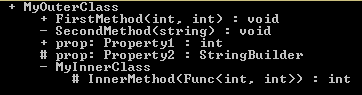
\includegraphics[scale=1]{syntaxwalker-results}
\caption[Displaying member layout with a SyntaxWalker]{Displaying member layout with a SyntaxWalker}
\label{syntaxwalker-results}
\end{figure}


